\channelmark{$\overline{\mathrm{ph}}$}
\mbox{$\displaystyle -\,$\,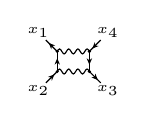
\begin{tikzpicture}[x=0.340cm, y=0.340cm, line width=0.420pt, baseline={([yshift=-0.6ex]0,0)}]
  \draw (-0.600,-0.375) -- (-0.600,0.375);
  \fill (-0.600,0.119) -- (-0.702,-0.119) -- (-0.600,-0.042) -- (-0.498,-0.119) -- cycle;
  \draw (0.600,0.375) -- (0.600,-0.375);
  \fill (0.600,-0.119) -- (0.702,0.119) -- (0.600,0.042) -- (0.498,0.119) -- cycle;
  \draw plot[smooth, tension=0.7] coordinates {(-0.600,0.375) (-0.557,0.440) (-0.514,0.468) (-0.471,0.440) (-0.429,0.375) (-0.386,0.310) (-0.343,0.282) (-0.300,0.310) (-0.257,0.375) (-0.214,0.440) (-0.171,0.468) (-0.129,0.440) (-0.086,0.375) (-0.043,0.310) (0.000,0.282) (0.043,0.310) (0.086,0.375) (0.129,0.440) (0.171,0.468) (0.214,0.440) (0.257,0.375) (0.300,0.310) (0.343,0.282) (0.386,0.310) (0.429,0.375) (0.471,0.440) (0.514,0.468) (0.557,0.440) (0.600,0.375)};
  \draw plot[smooth, tension=0.7] coordinates {(-0.600,-0.375) (-0.557,-0.310) (-0.514,-0.282) (-0.471,-0.310) (-0.429,-0.375) (-0.386,-0.440) (-0.343,-0.468) (-0.300,-0.440) (-0.257,-0.375) (-0.214,-0.310) (-0.171,-0.282) (-0.129,-0.310) (-0.086,-0.375) (-0.043,-0.440) (0.000,-0.468) (0.043,-0.440) (0.086,-0.375) (0.129,-0.310) (0.171,-0.282) (0.214,-0.310) (0.257,-0.375) (0.300,-0.440) (0.343,-0.468) (0.386,-0.440) (0.429,-0.375) (0.471,-0.310) (0.514,-0.282) (0.557,-0.310) (0.600,-0.375)};
  \draw (-0.600,0.375) -- (-1.024,0.799);
  \fill (-0.918,0.693) -- (-0.821,0.452) -- (-0.804,0.579) -- (-0.677,0.596) -- cycle;
  \draw (-0.600,-0.375) -- (-1.024,-0.799);
  \fill (-0.706,-0.481) -- (-0.947,-0.578) -- (-0.820,-0.595) -- (-0.803,-0.722) -- cycle;
  \draw (0.600,-0.375) -- (1.024,-0.799);
  \fill (0.918,-0.693) -- (0.821,-0.452) -- (0.804,-0.579) -- (0.677,-0.596) -- cycle;
  \draw (0.600,0.375) -- (1.024,0.799);
  \fill (0.706,0.481) -- (0.947,0.578) -- (0.820,0.595) -- (0.803,0.722) -- cycle;
  \fill (-0.600,0.375) circle (0.064);
  \fill (-0.600,-0.375) circle (0.064);
  \fill (0.600,-0.375) circle (0.064);
  \fill (0.600,0.375) circle (0.064);
  \node[font=\tiny, inner sep=0pt, anchor=315] at (-1.088,0.863) {$x_{1}$};
  \node[font=\tiny, inner sep=0pt, anchor=45] at (-1.088,-0.863) {$x_{2}$};
  \node[font=\tiny, inner sep=0pt, anchor=135] at (1.088,-0.863) {$x_{3}$};
  \node[font=\tiny, inner sep=0pt, anchor=225] at (1.088,0.863) {$x_{4}$};
\end{tikzpicture}}
\diagramgap
\mbox{$\displaystyle +\,$\,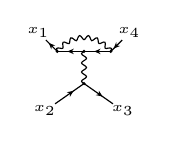
\begin{tikzpicture}[x=0.340cm, y=0.340cm, line width=0.420pt, baseline={([yshift=-0.6ex]0,0)}]
  \draw (0.000,0.300) -- (-1.000,0.300);
  \fill (-0.619,0.300) -- (-0.381,0.198) -- (-0.458,0.300) -- (-0.381,0.402) -- cycle;
  \draw (1.000,0.300) -- (0.000,0.300);
  \fill (0.381,0.300) -- (0.619,0.198) -- (0.542,0.300) -- (0.619,0.402) -- cycle;
  \draw plot[smooth, tension=0.7] coordinates {(-1.000,0.300) (-1.023,0.366) (-1.017,0.413) (-0.972,0.430) (-0.902,0.422) (-0.834,0.410) (-0.792,0.419) (-0.781,0.462) (-0.790,0.530) (-0.796,0.600) (-0.777,0.644) (-0.730,0.649) (-0.665,0.623) (-0.602,0.595) (-0.558,0.593) (-0.537,0.631) (-0.529,0.700) (-0.516,0.769) (-0.488,0.807) (-0.441,0.799) (-0.384,0.758) (-0.330,0.715) (-0.288,0.702) (-0.258,0.734) (-0.233,0.798) (-0.204,0.861) (-0.166,0.891) (-0.122,0.872) (-0.078,0.818) (-0.037,0.762) (0.000,0.739) (0.037,0.762) (0.078,0.818) (0.122,0.872) (0.166,0.891) (0.204,0.861) (0.233,0.798) (0.258,0.734) (0.288,0.702) (0.330,0.715) (0.384,0.758) (0.441,0.799) (0.488,0.807) (0.516,0.769) (0.529,0.700) (0.537,0.631) (0.558,0.593) (0.602,0.595) (0.665,0.623) (0.730,0.649) (0.777,0.644) (0.796,0.600) (0.790,0.530) (0.781,0.462) (0.792,0.419) (0.834,0.410) (0.902,0.422) (0.972,0.430) (1.017,0.413) (1.023,0.366) (1.000,0.300)};
  \draw plot[smooth, tension=0.7] coordinates {(0.000,-0.900) (-0.065,-0.857) (-0.093,-0.814) (-0.065,-0.771) (0.000,-0.729) (0.065,-0.686) (0.093,-0.643) (0.065,-0.600) (0.000,-0.557) (-0.065,-0.514) (-0.093,-0.471) (-0.065,-0.429) (0.000,-0.386) (0.065,-0.343) (0.093,-0.300) (0.065,-0.257) (0.000,-0.214) (-0.065,-0.171) (-0.093,-0.129) (-0.065,-0.086) (0.000,-0.043) (0.065,0.000) (0.093,0.043) (0.065,0.086) (0.000,0.129) (-0.065,0.171) (-0.093,0.214) (-0.065,0.257) (0.000,0.300)};
  \draw (-1.000,0.300) -- (-1.424,0.724);
  \fill (-1.318,0.618) -- (-1.221,0.377) -- (-1.204,0.504) -- (-1.077,0.521) -- cycle;
  \draw (0.000,-0.900) -- (-1.081,-1.657);
  \fill (-0.389,-1.172) -- (-0.643,-1.226) -- (-0.521,-1.265) -- (-0.526,-1.393) -- cycle;
  \draw (0.000,-0.900) -- (1.081,-1.657);
  \fill (0.693,-1.385) -- (0.555,-1.164) -- (0.560,-1.292) -- (0.438,-1.332) -- cycle;
  \draw (1.000,0.300) -- (1.424,0.724);
  \fill (1.106,0.406) -- (1.347,0.503) -- (1.220,0.520) -- (1.203,0.647) -- cycle;
  \fill (-1.000,0.300) circle (0.064);
  \fill (0.000,-0.900) circle (0.064);
  \fill (1.000,0.300) circle (0.064);
  \fill (0.000,0.300) circle (0.064);
  \node[font=\tiny, inner sep=0pt, anchor=315] at (-1.488,0.788) {$x_{1}$};
  \node[font=\tiny, inner sep=0pt, anchor=35] at (-1.155,-1.709) {$x_{2}$};
  \node[font=\tiny, inner sep=0pt, anchor=145] at (1.155,-1.709) {$x_{3}$};
  \node[font=\tiny, inner sep=0pt, anchor=225] at (1.488,0.788) {$x_{4}$};
\end{tikzpicture}}
\diagramgap
\mbox{$\displaystyle +\,$\,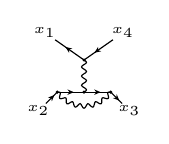
\begin{tikzpicture}[x=0.340cm, y=0.340cm, line width=0.420pt, baseline={([yshift=-0.6ex]0,0)}]
  \draw (0.000,-0.300) -- (1.000,-0.300);
  \fill (0.619,-0.300) -- (0.381,-0.198) -- (0.458,-0.300) -- (0.381,-0.402) -- cycle;
  \draw (-1.000,-0.300) -- (0.000,-0.300);
  \fill (-0.381,-0.300) -- (-0.619,-0.198) -- (-0.542,-0.300) -- (-0.619,-0.402) -- cycle;
  \draw plot[smooth, tension=0.7] coordinates {(0.000,0.900) (0.065,0.857) (0.093,0.814) (0.065,0.771) (0.000,0.729) (-0.065,0.686) (-0.093,0.643) (-0.065,0.600) (0.000,0.557) (0.065,0.514) (0.093,0.471) (0.065,0.429) (0.000,0.386) (-0.065,0.343) (-0.093,0.300) (-0.065,0.257) (0.000,0.214) (0.065,0.171) (0.093,0.129) (0.065,0.086) (0.000,0.043) (-0.065,0.000) (-0.093,-0.043) (-0.065,-0.086) (0.000,-0.129) (0.065,-0.171) (0.093,-0.214) (0.065,-0.257) (0.000,-0.300)};
  \draw plot[smooth, tension=0.7] coordinates {(-1.000,-0.300) (-0.931,-0.297) (-0.890,-0.312) (-0.885,-0.355) (-0.902,-0.422) (-0.917,-0.490) (-0.904,-0.536) (-0.858,-0.547) (-0.790,-0.530) (-0.724,-0.510) (-0.680,-0.514) (-0.664,-0.554) (-0.665,-0.623) (-0.661,-0.693) (-0.638,-0.734) (-0.590,-0.733) (-0.529,-0.700) (-0.470,-0.663) (-0.427,-0.656) (-0.401,-0.691) (-0.384,-0.758) (-0.363,-0.825) (-0.330,-0.859) (-0.284,-0.846) (-0.233,-0.798) (-0.185,-0.748) (-0.145,-0.729) (-0.111,-0.757) (-0.078,-0.818) (-0.041,-0.877) (0.000,-0.901) (0.041,-0.877) (0.078,-0.818) (0.111,-0.757) (0.145,-0.729) (0.185,-0.748) (0.233,-0.798) (0.284,-0.846) (0.330,-0.859) (0.363,-0.825) (0.384,-0.758) (0.401,-0.691) (0.427,-0.656) (0.470,-0.663) (0.529,-0.700) (0.590,-0.733) (0.638,-0.734) (0.661,-0.693) (0.665,-0.623) (0.664,-0.554) (0.680,-0.514) (0.724,-0.510) (0.790,-0.530) (0.858,-0.547) (0.904,-0.536) (0.917,-0.490) (0.902,-0.422) (0.885,-0.355) (0.890,-0.312) (0.931,-0.297) (1.000,-0.300)};
  \draw (0.000,0.900) -- (-1.081,1.657);
  \fill (-0.693,1.385) -- (-0.555,1.164) -- (-0.560,1.292) -- (-0.438,1.332) -- cycle;
  \draw (-1.000,-0.300) -- (-1.424,-0.724);
  \fill (-1.106,-0.406) -- (-1.347,-0.503) -- (-1.220,-0.520) -- (-1.203,-0.647) -- cycle;
  \draw (1.000,-0.300) -- (1.424,-0.724);
  \fill (1.318,-0.618) -- (1.221,-0.377) -- (1.204,-0.504) -- (1.077,-0.521) -- cycle;
  \draw (0.000,0.900) -- (1.081,1.657);
  \fill (0.389,1.172) -- (0.643,1.226) -- (0.521,1.265) -- (0.526,1.393) -- cycle;
  \fill (0.000,0.900) circle (0.064);
  \fill (-1.000,-0.300) circle (0.064);
  \fill (1.000,-0.300) circle (0.064);
  \fill (0.000,-0.300) circle (0.064);
  \node[font=\tiny, inner sep=0pt, anchor=325] at (-1.155,1.709) {$x_{1}$};
  \node[font=\tiny, inner sep=0pt, anchor=45] at (-1.488,-0.788) {$x_{2}$};
  \node[font=\tiny, inner sep=0pt, anchor=135] at (1.488,-0.788) {$x_{3}$};
  \node[font=\tiny, inner sep=0pt, anchor=215] at (1.155,1.709) {$x_{4}$};
\end{tikzpicture}}
\diagramgap
\mbox{$\displaystyle -\,$\,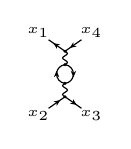
\begin{tikzpicture}[x=0.340cm, y=0.340cm, line width=0.420pt, baseline={([yshift=-0.6ex]0,0)}]
  \draw (0.000,-0.350) arc[start angle=263.974, end angle=96.026, radius=0.352];
  \fill (-0.315,0.119) -- (-0.417,-0.119) -- (-0.315,-0.042) -- (-0.213,-0.119) -- cycle;
  \draw (0.000,0.350) arc[start angle=83.974, end angle=-83.974, radius=0.352];
  \fill (0.315,-0.119) -- (0.417,0.119) -- (0.315,0.042) -- (0.213,0.119) -- cycle;
  \draw plot[smooth, tension=0.7] coordinates {(0.000,0.850) (0.064,0.808) (0.090,0.767) (0.064,0.725) (0.000,0.683) (-0.064,0.642) (-0.090,0.600) (-0.064,0.558) (0.000,0.517) (0.064,0.475) (0.090,0.433) (0.064,0.392) (0.000,0.350)};
  \draw plot[smooth, tension=0.7] coordinates {(0.000,-0.850) (-0.064,-0.808) (-0.090,-0.767) (-0.064,-0.725) (0.000,-0.683) (0.064,-0.642) (0.090,-0.600) (0.064,-0.558) (0.000,-0.517) (-0.064,-0.475) (-0.090,-0.433) (-0.064,-0.392) (0.000,-0.350)};
  \draw (0.000,0.850) -- (-0.614,1.280);
  \fill (-0.436,1.155) -- (-0.299,0.935) -- (-0.304,1.063) -- (-0.182,1.102) -- cycle;
  \draw (0.000,-0.850) -- (-0.614,-1.280);
  \fill (-0.179,-0.975) -- (-0.433,-1.028) -- (-0.311,-1.068) -- (-0.316,-1.196) -- cycle;
  \draw (0.000,-0.850) -- (0.614,-1.280);
  \fill (0.436,-1.155) -- (0.299,-0.935) -- (0.304,-1.063) -- (0.182,-1.102) -- cycle;
  \draw (0.000,0.850) -- (0.614,1.280);
  \fill (0.179,0.975) -- (0.433,1.028) -- (0.311,1.068) -- (0.316,1.196) -- cycle;
  \fill (0.000,0.850) circle (0.064);
  \fill (0.000,-0.850) circle (0.064);
  \fill (0.000,0.350) circle (0.064);
  \fill (0.000,-0.350) circle (0.064);
  \node[font=\tiny, inner sep=0pt, anchor=325] at (-0.688,1.332) {$x_{1}$};
  \node[font=\tiny, inner sep=0pt, anchor=35] at (-0.688,-1.332) {$x_{2}$};
  \node[font=\tiny, inner sep=0pt, anchor=145] at (0.688,-1.332) {$x_{3}$};
  \node[font=\tiny, inner sep=0pt, anchor=215] at (0.688,1.332) {$x_{4}$};
\end{tikzpicture}}
\break
\channelmark{$\mathrm{pp}$}
\mbox{$\displaystyle +\,$\,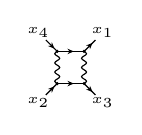
\begin{tikzpicture}[x=0.340cm, y=0.340cm, line width=0.420pt, baseline={([yshift=-0.6ex]0,0)}]
  \draw (-0.500,0.600) -- (0.500,0.600);
  \fill (0.119,0.600) -- (-0.119,0.702) -- (-0.042,0.600) -- (-0.119,0.498) -- cycle;
  \draw (-0.500,-0.600) -- (0.500,-0.600);
  \fill (0.119,-0.600) -- (-0.119,-0.498) -- (-0.042,-0.600) -- (-0.119,-0.702) -- cycle;
  \draw plot[smooth, tension=0.7] coordinates {(0.500,0.600) (0.565,0.557) (0.593,0.514) (0.565,0.471) (0.500,0.429) (0.435,0.386) (0.407,0.343) (0.435,0.300) (0.500,0.257) (0.565,0.214) (0.593,0.171) (0.565,0.129) (0.500,0.086) (0.435,0.043) (0.407,0.000) (0.435,-0.043) (0.500,-0.086) (0.565,-0.129) (0.593,-0.171) (0.565,-0.214) (0.500,-0.257) (0.435,-0.300) (0.407,-0.343) (0.435,-0.386) (0.500,-0.429) (0.565,-0.471) (0.593,-0.514) (0.565,-0.557) (0.500,-0.600)};
  \draw plot[smooth, tension=0.7] coordinates {(-0.500,-0.600) (-0.565,-0.557) (-0.593,-0.514) (-0.565,-0.471) (-0.500,-0.429) (-0.435,-0.386) (-0.407,-0.343) (-0.435,-0.300) (-0.500,-0.257) (-0.565,-0.214) (-0.593,-0.171) (-0.565,-0.129) (-0.500,-0.086) (-0.435,-0.043) (-0.407,0.000) (-0.435,0.043) (-0.500,0.086) (-0.565,0.129) (-0.593,0.171) (-0.565,0.214) (-0.500,0.257) (-0.435,0.300) (-0.407,0.343) (-0.435,0.386) (-0.500,0.429) (-0.565,0.471) (-0.593,0.514) (-0.565,0.557) (-0.500,0.600)};
  \draw (0.500,0.600) -- (0.924,1.024);
  \fill (0.818,0.918) -- (0.577,0.821) -- (0.704,0.804) -- (0.721,0.677) -- cycle;
  \draw (-0.500,-0.600) -- (-0.924,-1.024);
  \fill (-0.606,-0.706) -- (-0.847,-0.803) -- (-0.720,-0.820) -- (-0.703,-0.947) -- cycle;
  \draw (0.500,-0.600) -- (0.924,-1.024);
  \fill (0.818,-0.918) -- (0.721,-0.677) -- (0.704,-0.804) -- (0.577,-0.821) -- cycle;
  \draw (-0.500,0.600) -- (-0.924,1.024);
  \fill (-0.606,0.706) -- (-0.703,0.947) -- (-0.720,0.820) -- (-0.847,0.803) -- cycle;
  \fill (0.500,0.600) circle (0.064);
  \fill (-0.500,-0.600) circle (0.064);
  \fill (0.500,-0.600) circle (0.064);
  \fill (-0.500,0.600) circle (0.064);
  \node[font=\tiny, inner sep=0pt, anchor=225] at (0.988,1.088) {$x_{1}$};
  \node[font=\tiny, inner sep=0pt, anchor=45] at (-0.988,-1.088) {$x_{2}$};
  \node[font=\tiny, inner sep=0pt, anchor=135] at (0.988,-1.088) {$x_{3}$};
  \node[font=\tiny, inner sep=0pt, anchor=315] at (-0.988,1.088) {$x_{4}$};
\end{tikzpicture}}
\diagramgap
\mbox{$\displaystyle -\,$\,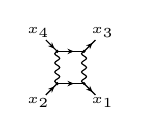
\begin{tikzpicture}[x=0.340cm, y=0.340cm, line width=0.420pt, baseline={([yshift=-0.6ex]0,0)}]
  \draw (-0.500,-0.600) -- (0.500,-0.600);
  \fill (0.119,-0.600) -- (-0.119,-0.498) -- (-0.042,-0.600) -- (-0.119,-0.702) -- cycle;
  \draw (-0.500,0.600) -- (0.500,0.600);
  \fill (0.119,0.600) -- (-0.119,0.702) -- (-0.042,0.600) -- (-0.119,0.498) -- cycle;
  \draw plot[smooth, tension=0.7] coordinates {(0.500,-0.600) (0.435,-0.557) (0.407,-0.514) (0.435,-0.471) (0.500,-0.429) (0.565,-0.386) (0.593,-0.343) (0.565,-0.300) (0.500,-0.257) (0.435,-0.214) (0.407,-0.171) (0.435,-0.129) (0.500,-0.086) (0.565,-0.043) (0.593,0.000) (0.565,0.043) (0.500,0.086) (0.435,0.129) (0.407,0.171) (0.435,0.214) (0.500,0.257) (0.565,0.300) (0.593,0.343) (0.565,0.386) (0.500,0.429) (0.435,0.471) (0.407,0.514) (0.435,0.557) (0.500,0.600)};
  \draw plot[smooth, tension=0.7] coordinates {(-0.500,-0.600) (-0.565,-0.557) (-0.593,-0.514) (-0.565,-0.471) (-0.500,-0.429) (-0.435,-0.386) (-0.407,-0.343) (-0.435,-0.300) (-0.500,-0.257) (-0.565,-0.214) (-0.593,-0.171) (-0.565,-0.129) (-0.500,-0.086) (-0.435,-0.043) (-0.407,0.000) (-0.435,0.043) (-0.500,0.086) (-0.565,0.129) (-0.593,0.171) (-0.565,0.214) (-0.500,0.257) (-0.435,0.300) (-0.407,0.343) (-0.435,0.386) (-0.500,0.429) (-0.565,0.471) (-0.593,0.514) (-0.565,0.557) (-0.500,0.600)};
  \draw (0.500,-0.600) -- (0.924,-1.024);
  \fill (0.818,-0.918) -- (0.721,-0.677) -- (0.704,-0.804) -- (0.577,-0.821) -- cycle;
  \draw (-0.500,-0.600) -- (-0.924,-1.024);
  \fill (-0.606,-0.706) -- (-0.847,-0.803) -- (-0.720,-0.820) -- (-0.703,-0.947) -- cycle;
  \draw (0.500,0.600) -- (0.924,1.024);
  \fill (0.818,0.918) -- (0.577,0.821) -- (0.704,0.804) -- (0.721,0.677) -- cycle;
  \draw (-0.500,0.600) -- (-0.924,1.024);
  \fill (-0.606,0.706) -- (-0.703,0.947) -- (-0.720,0.820) -- (-0.847,0.803) -- cycle;
  \fill (0.500,-0.600) circle (0.064);
  \fill (-0.500,-0.600) circle (0.064);
  \fill (0.500,0.600) circle (0.064);
  \fill (-0.500,0.600) circle (0.064);
  \node[font=\tiny, inner sep=0pt, anchor=135] at (0.988,-1.088) {$x_{1}$};
  \node[font=\tiny, inner sep=0pt, anchor=45] at (-0.988,-1.088) {$x_{2}$};
  \node[font=\tiny, inner sep=0pt, anchor=225] at (0.988,1.088) {$x_{3}$};
  \node[font=\tiny, inner sep=0pt, anchor=315] at (-0.988,1.088) {$x_{4}$};
\end{tikzpicture}}
